\documentclass[12pt]{article}
\usepackage{graphicx}
\usepackage{enumitem}
\usepackage{amsmath}
\usepackage{gvv-book}
\usepackage{gvv}

\title{\textbf{2.3.11}}
\author{\textbf{EE25BTECH11008 - Anirudh M Abhilash}}
\date{September 14, 2025}

\begin{document}

\maketitle
\section*{Question}

Find the acute angle between the planes 
\begin{align*}
x - 2y - 2z = 5 \\
\quad 3x - 6y + 2z = 7
\end{align*}

\section*{Solution}

The angle between two planes is the angle between their normals.
Let
\[
\vec{n}_1 = \myvec{1 \\ -2 \\ -2}, 
\quad \vec{n}_2 = \myvec{3 \\ -6 \\ 2}.
\]

The dot product is
\begin{align}
\vec{n}_1^\top \vec{n}_2 &= 1\cdot 3 + (-2)(-6) + (-2)(2) \\
&= 3 + 12 - 4 \\
&= 11.
\end{align}

The norms are
\begin{align}
\|\vec{n}_1\| &= \sqrt{1^2 + (-2)^2 + (-2)^2} = \sqrt{9} = 3, \\
\|\vec{n}_2\| &= \sqrt{3^2 + (-6)^2 + 2^2} = \sqrt{49} = 7.
\end{align}

Hence,
\begin{align}
\cos\theta &= \frac{\vec{n}_1^\top \vec{n}_2}{\|\vec{n}_1\|\|\vec{n}_2\|} \\
&= \frac{11}{3\cdot 7} \\
&= \frac{11}{21}.
\end{align}

Therefore, the acute angle between the planes is
\[
\boxed{\theta = \arccos\!\left(\tfrac{11}{21}\right) \approx 58.41^\circ}
\]

\begin{figure}[H]\centering
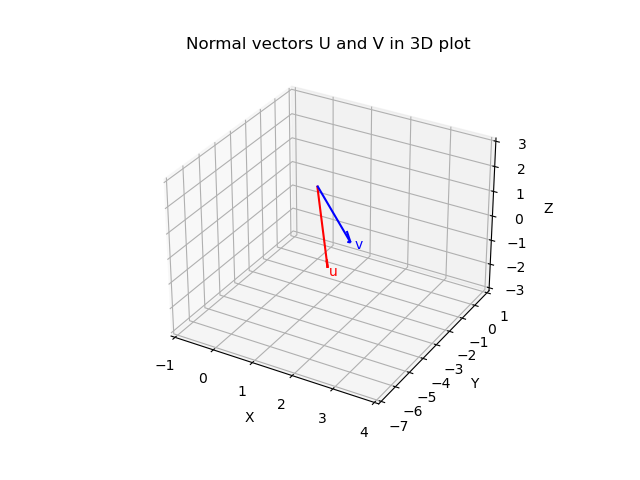
\includegraphics[width=1\columnwidth]{figs/plt.png}
\caption{Normal vectors $\vec{U}$ and $\vec{V}$}
\label{fig:plt}
\end{figure}

\end{document}
